\section{Results}
The results given in this section aim to demonstrate how the proposed method can be used to find a scalable solution to the bus charge problem. Because the proposed solution contains various sub-problems, optimization parameters for each sub-problem may be tuned to best meet the demands of a given scenario, allowing for a wide degree of flexability that is not present in prior works which formulate solutions to the bus charge problem as a single program.
\subsection{Overall Performance}
In this section, we compare the proposed method with a baseline algorithm and a method developed be \textcolor{red}{insert reference to He. et al here}. The baseline method models how bus drivers charge their electric vehicles at the Utah Transit Authority in Salt Lake City, Utah. At UTA, when bus drivers arrive at the station, they refuel their electric buses whenever a charger is available so that the number of charge sessions is maximized. The method from \textcolor{red}{He et al.} works somewhat differently by minimising the cost of energy with respect to the time of use tarrifs $\mu_{e-on}$ and $\mu_{e-off}$.
\par The comparison we observe is given for a 10-bus, 10-charger scenario and a single group. Each method was used to compute a charage schedule and the costs from demand, facilities, and energy charges are given in Fig. \ref{fig:results:costComparison}. Note how the baseline algorithm suffers significantly from the demand charges associated with On-Peak Power, and \textcolor{red}{He et al.} incurres additional cost from the facilities charges, indicating that an emphasis on energy charges and habitual charging patterns can be improved.
\par We observe where the differences in cost originate in Fig. \ref{fig:results:totalPower}. Observe how the baseline charge profile achieved the largest 15-minute average power between 19:12 adn 21:36 which is during on-peak hours and consequently yielded the large On-Peak Power charges given in Fig. \ref{fig:results:costComparison}. Additionally, note how the proposed method maintains a relatively flat power profile so that the load is balanced throughout the day which we investigate in Fig. \ref{fig:results:powerPlot}.
\par In Fig. \ref{fig:results:powerPlot}, note how the proposed method produces a bus load that mirrors the uncontrolled load, yielding the flat load profile from Fig. \ref{fig:results:totalPower} which is especially prevalent from 7:12 to 14:24. The results show that the proposed method works well, outperforming both historical patterns at UTA as well and improves upon prior academic techniques.
\begin{figure}
	\centering
	\makeComparisonBarChartThree{media/11_results/costComparison.csv}{Cost (Dollars)}{Baseline}{He et al.}{Proposed}
	\caption{Cost comparison with prior work}
	\label{fig:results:costComparison}
\end{figure} 

 
\begin{figure*}
	\centering
	\makeComparisonPower{media/11_results/powerPlotfiscal.csv}{media/11_results/powerPlotconsumption.csv}{15-Minute Average Power (kW)}{Proposed}{He et al.}
	\caption{Comparison between uncontrolled and bus loads}
	\label{fig:results:powerPlot}
\end{figure*}


\begin{figure*}
	\centering
	\makeComparisonTotalPower{media/11_results/totalPowerfiscalproTime.csv}{media/11_results/totalPowerconsumptionproTime.csv}{15-Minute Average Power (kW)}{Proposed}{He et al.}
	\caption{15-Minute average power for one day}
	\label{fig:results:totalPower}
\end{figure*}


\subsection{Optimality Gaps and Contention}
In the previous section, we discussed performance of the proposed method when each program is solved to an optimal solution. In general, the most computationally demanding solution addressed bus-to-charger placement and generally requries a gap of $1\times10^{-5}$ for optimality. This work also seeks to address how to compute a solution in a scalable manner and so this section reviews computational time as the number of buses increases.  
\par This section considers a 7-charger scenario and compares runtime results for 8, 9, and 10 buses to illustrate how runtimes for set optimality gaps change as contention increases. Fig. \ref{fig:results:scalabilityTimeVsGap} shows how the computational time increases as the optimality gap decreases. Note how the computational time suddenly increases as the gap decreases, a phenomena which is exacerbated as contention increases. Additionally, note that the optimality gaps are small even before the sudden increase in runtime indicating that it may not be necessary to solve past the turning point where the runtime suddenly increases. 
\begin{figure}
\centering
\begin{tikzpicture}
	\pgfplotstableread[col sep=comma]{\rootdirectorythree/media/11_results/avgPowerVsDurationOpt.csv}\tableOpt
	\pgfplotstableread[col sep=comma]{\rootdirectorythree/media/11_results/avgPowerVsDurationDis.csv}\tableDis
	\begin{axis}[ylabel=Duration (Seconds), xlabel=Average Power (kWh), ymode=log]
		\addplot[blue!20, draw=blue, only marks,mark size=1pt] table[x=avgPower, y=duration] {\tableOpt};
		\addplot[red!20, draw=red, only marks,mark size=1pt] table[x=avgPower, y=duration] {\tableDis};
		\legend{Optimal Solution, Relaxed Optimality Gap}
	\end{axis}
\end{tikzpicture}
\caption{Comparison of charge session duration vs average charge rate}
\label{fig:results:sessionComparison}
\end{figure}
 
\begin{figure}
	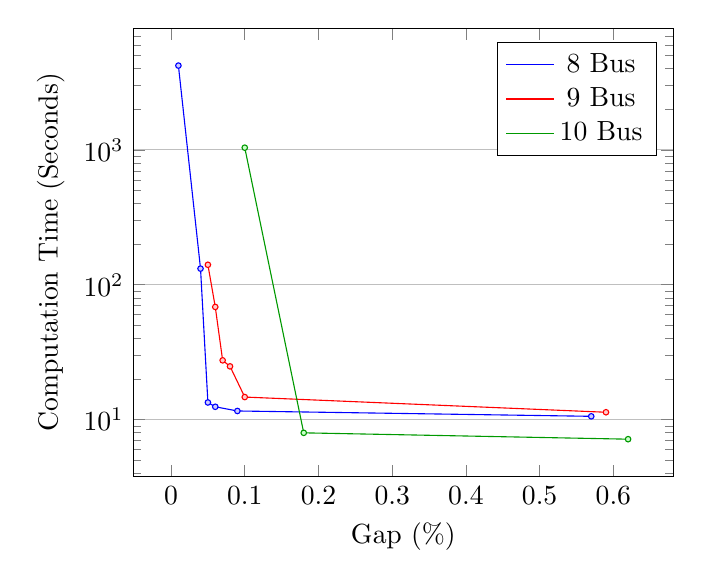
\begin{tikzpicture}
		\begin{axis}[ymajorgrids=true, ylabel={Computation Time (Seconds)}, ymode=log, xlabel={Gap (\%)}, legend pos=north east]%, xtick={0.1, 0.05, 0.01, 0.005, 0.001, 0.0005, 0.0001, 0.00005, 0.00001, 0.000005, 0.000001}, xticklabels={$1\times10^{-1}$, $5\times10^{-2}$, $1\times10^{-2}$, $5\times10^{-3}$, $1\times10^{-3}$, $5\times10^{-4}$, $1\times10^{-4}$, $5\times10^{-5}$, $1\times10^{-5}$, $5\times10^{-6}$, $1\times10^{-6}$}]
			\addplot[blue] coordinates {
				(0.57, 10.58)
				(0.09, 11.59)
				(0.06, 12.45)
				(0.05, 13.40)
				(0.04, 131.78)
				(0.01, 4223.25)
			};
			\addplot[red] coordinates {
				(0.59, 11.34)
				(0.10, 14.70)
				(0.08, 24.83)
				(0.07, 27.51)
				(0.06, 68.49)
				(0.05, 140.70)
			};
			\addplot[green!60!black] coordinates {
				(0.62, 7.16)
				(0.18, 7.98)
				(0.10, 1039.33)
			}; 
			\addplot[fill=blue!20, draw=blue, only marks, mark size=1pt] coordinates {
				(0.57, 10.58)
				(0.09, 11.59)
				(0.06, 12.45)
				(0.05, 13.40)
				(0.04, 131.78)
				(0.01, 4223.25)}; 
			\addplot[fill=red!20, draw=red, only marks, mark size=1pt] coordinates {
				(0.59, 11.34)
				(0.10, 14.70)
				(0.08, 24.83)
				(0.07, 27.51)
				(0.06, 68.49)
				(0.05, 140.70)
			}; 
			\addplot[fill=green!20, draw=green!60!black, only marks, mark size=1pt] coordinates{
				(0.62, 7.16)
				(0.18, 7.98)
				(0.10, 1039.33) 
			};
	\legend{8 Bus, 9 Bus, 10 Bus};
		\end{axis}
	\end{tikzpicture}
	\caption{Comparison of Runtime for a 7-Charger Scenario}
	\label{fig:results:scalabilityTimeVsGap}
\end{figure}



\subsection{Contention: Sub-Optimal Schedules}
In the previous section we observed that the proposed method cannot scale with contention if the optimality gap dips below the turning point where runtime suddenly increases. In this section, we show that a relaxed optimality gap in the charger placement problem may result in an undesirable solution and consequently that there exist scenarios that require small optimality gaps which normally lie beyond the turning point shown in Fig. \ref{fig:results:scalabilityTimeVsGap}, indicating the need to reduce the charger assignment problem's computational complexity. 
\par Fig. \ref{fig:results:sessionComparison} displays the charge session durations as a function of average charge rate for two 18 bus 6 charger scenarios where the first was computed using a small optimality gap and the second resulted when the gap was relaxed. Note how the charge sessions from the optimal solution tend to have larger session durations and lower charge rates than the relaxed solution which is desired because sessions with low charge rates and long durations are simpler to carry out in practice. 
\par Figures \ref{fig:results:disoptimalRoutes} and \ref{fig:results:optimalRoutes} show the corresponding optimal and relaxed charge plans by letting the color at the $i,j$ location represent the charge rate for bus $i$ at time $j$ and show why an optimal solution to the charger assignment problem yields better charge sessions. Observe how the first sessions for buses 1 -- 4 and 6 -- 13 are assigned to a single charger in the relaxed solution, which compresses the charge sessions to accomodate the large number of buses while the remaining chargers appear to have one session at most. In comparison, the optimal solution in Fig. \ref{fig:results:optimalRoutes} has a more evenly distributed session load for each charger so that each session is lengthened, leading to lower charge rates. 
\par It is also interesting to note that the monthly costs of each solution may or may not be equivalent even though an optimal solution is clearly superior. Therefore, a small gap is required to consistently achieve optimal session placement. We also know from Fig. \ref{fig:results:scalabilityTimeVsGap} that small optimality gaps may increase the number of computations so that the charger assignment problem becomes untractable for large numbers of buses.  
\input{media/11_results/disoptimalRoutes.tex}
\input{media/11_results/sessionImageStyle}
\begin{figure*}
\begin{tikzpicture}
\begin{axis}[colorbar, ChargeSessionImage, width=0.95\textwidth, height=0.5\textwidth, point meta min=0, point meta max=350, xmin=0.5, xmax=4320.5,xtick={540, 1080, 1620, 2160, 2700, 3240, 3780, 4320}, xticklabels={3:00, 6:00, 9:00, 12:00, 15:00, 18:00, 21:00, 0:00}, ymin=0.5, ymax=18.5]

\addplot [forget plot] graphics [xmin=0.5, xmax=4320.5, ymin=0.5, ymax=18.5] {media/11_results/optimalRoutes-1.png};
\end{axis}

\end{tikzpicture}%
\caption{Routes with a small gap in the route placement problem}
\label{fig:results:optimalRoutes}
\end{figure*}
 

\subsection{The Importance of Groups}
One contribution this work provides is a {\it scalable} way to compute cost-oriented charge schedules. We know from the previous section that the charger assignment problem will not scale for small optimality gaps. This section describes how the computational complexity of the charger assignment problem can be managed by separating the buses into groups so that the charger assignment problem can be solved for each group independently. 
\par In this section, we consider a 18 bus, 12 charger scenario with a 0.13\% gap in the charger assignment problem. Fig. \ref{fig:results:groupResults}, shows the respective runtimes for a one and two group scenario as computed in Section \ref{sec:groupAssignment}. Note how the runtime for the two group scenario is several orders of magnitude less then the runtime for the single group case which demonstrates how a small number of groups can manage the runtime for optimal charger assignment solutions.
\begin{figure}
\centering
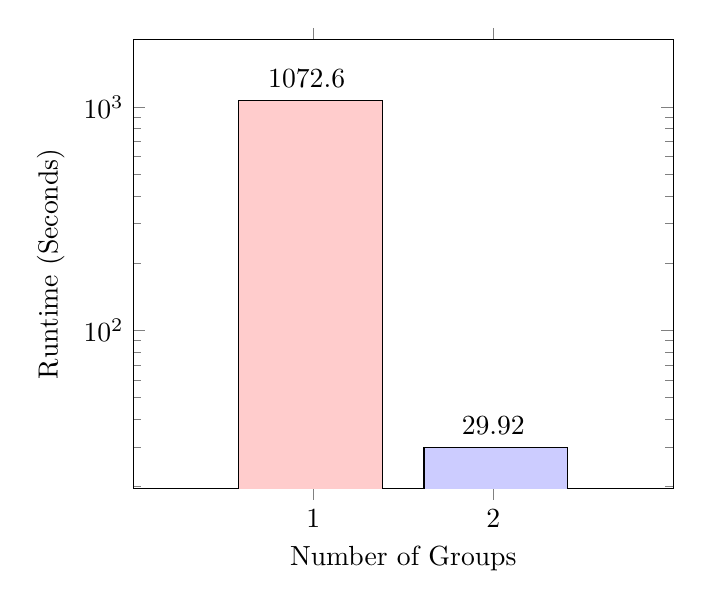
\begin{tikzpicture}
	\begin{axis}[ybar, ymode=log, ymax=2000, xmin=0, xmax=3, xtick={1,2}, xlabel=Number of Groups, ylabel=Runtime (Seconds)]
		\addplot[fill=red!20, bar width=0.8] coordinates {(1.4, 1072.6)};
		\addplot[fill=blue!20, bar width=0.8]  coordinates {(1.6, 29.92)};
	\end{axis}
	\node at (2.2,5.2){1072.6};
	\node at (4.57, 0.79){29.92};
\end{tikzpicture}
\caption{Runtimes for a 18 bus 12 charger scenario at a 0.13\% gap}
\label{fig:results:groupResults}
\end{figure}
 
\subsection{Effects of De-Fragmentation}
This paper also addresses the operational preference to consolidate charge sessions when possible. This section demonstrates the effectiveness of the defragmentation method given in Section \ref{sec:defragmentation} and how consolidation affects the monthly cost. In section \ref{sec:defragmentation}, the threshold for defragmentation is given by the minimum allowable energy per charge session. In this section we compare two 40 bus 7 charger scenarios where the first contains results without defragmentation and the second consolidates charge sessions so that each session delivers at least 30 kWh. The results for each session are presented in Figures \ref{fig:results:noFragmentationChargeLimit} and \ref{fig:results:defragmentedChargeLimit} where the color of $i,j$ element of a figure represents the charge rate for bus $i$ during time $j$. Note how Fig. \ref{fig:results:noFragmentationChargeLimit} contains {\it many} small an inconsequential charge sessions and requires each bus to charge each time it enters the station. In comparison, Fig. \ref{fig:results:defragmentedChargeLimit} contains only a handful of charge sessions so that each bus only need charge 4 -- 5 times throughout the day.  
\par Furthermore, Fig. \ref{fig:results:defragmentationCostProTime} demonstrates that despite the additional constraints associated with consolidation, the monthly cost remains consistent over a large window of thresholds. As the minimum allowable energy per session increases, the number of binary variables in the defragmentation problem increases, resulting in significant runtimes for the defragmentation problem as shown in Fig. \ref{fig:results:defragmentationTimeProTime}. However, because buses are divided into groups prior to defragmentation, the smaller groups decrease the computational complexity for defragmentation so that larger consolidation thresholds can be applied in a scalable manner. 
\begin{figure*}
\centering
\begin{tikzpicture} 
\begin{axis}[colorbar, ChargeSessionImage, width=5.2in, height=2in, point meta min=0, point meta max=350, xmin=0.5, xmax=4320.5, xtick={540, 1080, 1620, 2160, 2700, 3240, 3780, 4320}, xticklabels={3:00, 6:00, 9:00, 12:00, 15:00, 18:00, 21:00, 0:00}, ymin=0.5, ymax=40.5]
\addplot [forget plot] graphics [xmin=0.5, xmax=4320.5, ymin=0.5, ymax=40.5] {\rootdirectorythree/media/11_results/defragmentedChargeLimit-1.png}; 
\end{axis} 
\end{tikzpicture}
\caption{Routes with De-Fragmentation}
\label{fig:results:defragmentedChargeLimit}
\end{figure*}

\begin{figure*}
\centering
\begin{tikzpicture} 
\begin{axis}[colorbar, ChargeSessionImage, width=0.95\textwidth, height=0.5\textwidth, point meta min=0, point meta max=350, xmin=0.5, xmax=4320.5, xtick={540, 1080, 1620, 2160, 2700, 3240, 3780, 4320}, xticklabels={3:00, 6:00, 9:00, 12:00, 15:00, 18:00, 21:00, 0:00}, ymin=0.5, ymax=40.5]
\addplot [forget plot] graphics [xmin=0.5, xmax=4320.5, ymin=0.5, ymax=40.5] {media/11_results/noFragmentationChargeLimit-1.png}; 
\end{axis} 
\end{tikzpicture}
\caption{Routes without De-Fragmentation}
\label{fig:results:noFragmentationChargeLimit}
\end{figure*}
 
\begin{figure}\centering
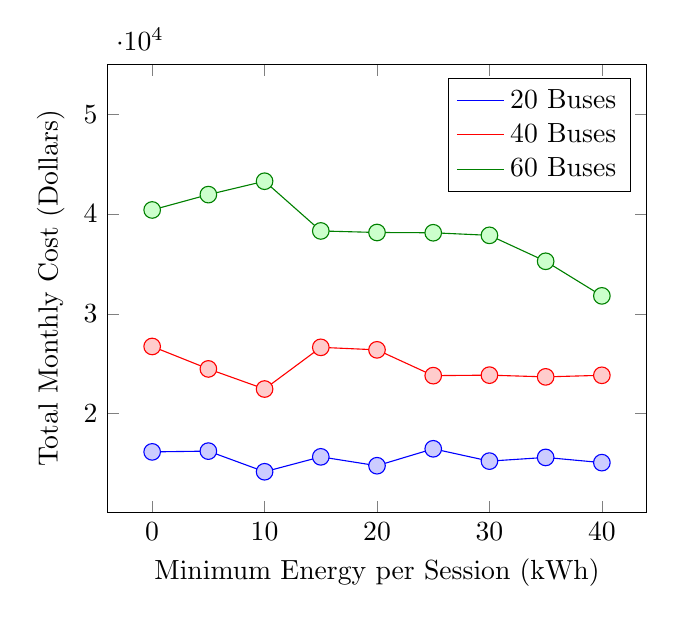
\begin{tikzpicture}
\begin{axis}[xlabel=Minimum Energy per Session (kWh), ylabel=Total Monthly Cost (Dollars), ymax=55000, legend pos=north east]
	\addplot[blue] coordinates {
		(0, 16183.79)   
	  (5, 16260.98)  
		(10,14194.10)  
		(15,15686.16)  
		(20,14798.53)  
		(25,16492.56)  
		(30,15259.19)  
		(35,15628.38)  
		(40,15106.82)};
\addplot[red] coordinates {
		(0, 26738.71)
		(5, 24491.03)
	  (10,22476.88)
		(15,26650.71)
		(20,26400.31)
		(25,23816.91)
		(30,23866.55)
		(35,23693.25)
		(40,23851.78)};
\addplot[green!50!black] coordinates {
		(0, 40405.72)
		(5, 41942.45)
	  (10,43284.09)
		(15,38304.96)
		(20,38150.28)
		(25,38122.51)
		(30,37864.79)
		(35,35268.11)
		(40,31805.12)};

\addplot[blue!20, draw=blue, only marks, mark size=3pt] coordinates {
		(0, 16183.79)  
		(5, 16260.98)  
	  (10,14194.10)  
		(15,15686.16)  
		(20,14798.53)  
		(25,16492.56)  
		(30,15259.19)  
		(35,15628.38)   
		(40,15106.82)};
\addplot[red!20, draw=red, only marks, mark size=3pt] coordinates {
	(0, 26738.71)  	
	(5, 24491.03)  	
	(10,22476.88)   
	(15,26650.71)  	
	(20,26400.31)  	
	(25,23816.91)  	
	(30,23866.55)  	
	(35,23693.25)  	
	(40,23851.78)};	
\addplot[green!20, draw=green!50!black, only marks, mark size=3pt] coordinates {
	(0, 40405.72)  
	(5, 41942.45)  
	(10,43284.09)  
	(15,38304.96)  
	(20,38150.28)  
	(25,38122.51)  
	(30,37864.79)  
	(35,35268.11)  
	(40,31805.12)};

\legend{20 Buses, 40 Buses, 60 Buses} 
\end{axis}
\end{tikzpicture}
\caption{Cost comparison of different degragmentation thresholds in a pro-time optimization scheme.}
\label{fig:results:defragmentationCostProTime}
\end{figure}

\begin{figure}
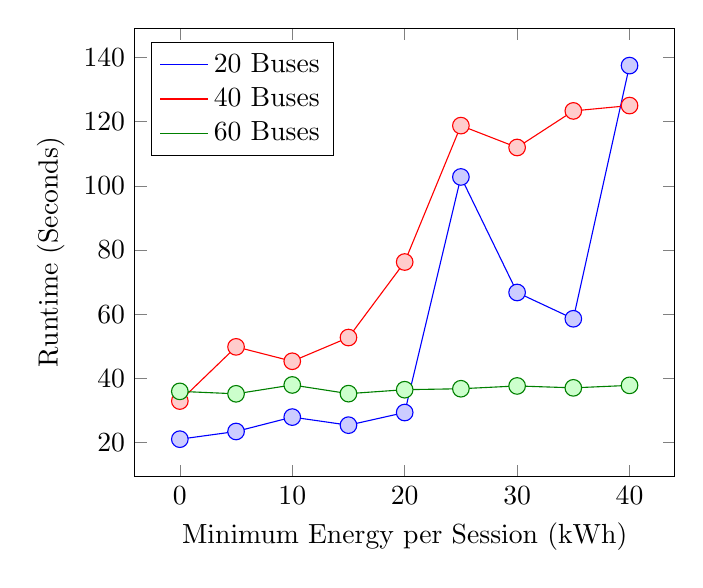
\begin{tikzpicture}
\begin{axis}[xlabel=Minimum Energy per Session (kWh), ylabel=Runtime (Seconds), legend pos=north west]
	\addplot[blue] coordinates {
		(0, 21.00)
		(5, 23.40)
	  (10,27.89)
		(15,25.37)
		(20,29.31)
		(25,102.78)
		(30,66.75)
		(35,58.55)
		(40,137.51)}; 
\addplot[red] coordinates {
		(0, 32.89)
		(5, 49.79)
	  (10,45.30)
		(15,52.70)
		(20,76.25)
		(25,118.79)
		(30,111.97)
		(35,123.37)
		(40,125.04)}; 
\addplot[green!50!black] coordinates {
		(0, 35.91)
		(5, 35.15)
	  (10,37.91)
		(15,35.20)
		(20,36.43)
		(25,36.73)
		(30,37.60)
		(35,37.01)
		(40,37.78)}; 
\addplot[blue!20, draw=blue, only marks, mark size=3pt] coordinates {
		(0, 21.00)
		(5, 23.40)
	  (10,27.89)
		(15,25.37)
		(20,29.31)
		(25,102.78)
		(30,66.75)
		(35,58.55)
		(40,137.51)}; 
\addplot[red!20, draw=red, only marks, mark size=3pt] coordinates {
		(0, 32.89)
		(5, 49.79)
	  (10,45.30)
		(15,52.70)
		(20,76.25)
		(25,118.79)
		(30,111.97)
		(35,123.37)
		(40,125.04)}; 
\addplot[green!20, draw=green!50!black, only marks, mark size=3pt] coordinates {
		(0, 35.91)
		(5, 35.15)
	  (10,37.91)
		(15,35.20)
		(20,36.43)
		(25,36.73)
		(30,37.60)
		(35,37.01)
		(40,37.78)}; 
\legend{20 Buses, 40 Buses, 60 Buses}		
\end{axis}
\end{tikzpicture}
\caption{Comparison of runtime for the uncontested and contested scenarios over different de-fragmentation criteria}
\label{fig:results:runtimeDefragmentation}
\end{figure}

\subsection{Scalability}
In this section, we consolidate what we have learned in the previous sections to demonstrate how the proposed framework can be used to compute a scalable and cost effective solution for large numbers of buses. This section focuses on a scenario with a minimum energy per session of 20 kWh, a relaxed gap for the charger assignment solution, and a single group.
\par The results given in Fig. \ref{fig:results:scalabilityRuntimes} show a runtime that generally increases by one second per bus from 10 to 110 buses.  One would expect the runtime to increase at least on the order of $O(n^2)$ for a globally optimal solution because of the coupling between bus variables. The fact that the proposed method appears linear on the given range indicates a scalable solution. 
\par Generally, one would also expect such savings to come with significant increases to the monthly cost. The results in Fig. \ref{fig:results:scalabilityCosts} however demonstrate how the proposed solution yields a quasi-linear increase of approximately \$404.10 dollars per bus per month. 
\begin{figure}
\centering
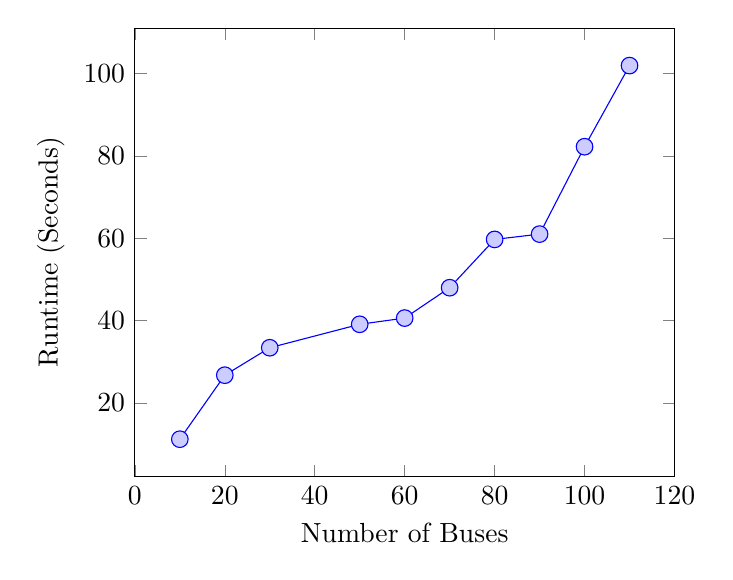
\begin{tikzpicture}
\begin{axis}[xlabel=Number of Buses, ylabel=Runtime (Seconds), legend pos=north west]
	\addplot[blue] coordinates {
		(10, 11.18)   
	  (20, 26.74)  
		(30, 33.41)  
		(50, 39.11)  
		(60, 40.62)  
		(70, 48.00)  
		(80, 59.74)  
		(90, 61.03)
		(100, 82.27)
		(110, 101.99)}; 
\addplot[blue!20, draw=blue, only marks, mark size=3pt] coordinates {
		(10, 11.18)   
	  (20, 26.74)  
		(30, 33.41)  
		(50, 39.11)  
		(60, 40.62)  
		(70, 48.00)  
		(80, 59.74)  
		(90, 61.03)
		(100, 82.27)
		(110, 101.99)};
\end{axis}
\end{tikzpicture}
\caption{Runtime comparison for different numbers of buses}
\label{fig:results:scalabilityRuntimes}
\end{figure}

\begin{figure}
\centering
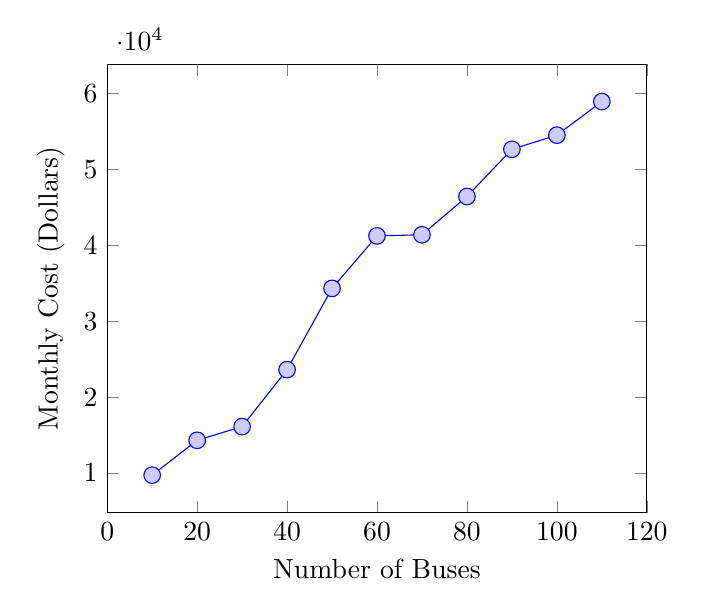
\begin{tikzpicture}
\begin{axis}[xlabel=Number of Buses, ylabel=Monthly Cost (Dollars), legend pos=north west]
	\addplot[blue] coordinates {
		(10, 9724.43)   
	  (20, 14312.58)  
		(30, 16113.51)  
		(40, 23617.81)
		(50, 34317.80)  
		(60, 41226.07)  
		(70, 41374.21) 
		(80, 46412.54)  
		(90, 52628.26)
		(100, 54490.15) 
		(110, 58912.91)}; 
\addplot[blue!20, draw=blue, only marks, mark size=3pt] coordinates {
		(10, 9724.43)   
	  (20, 14312.58)  
		(30, 16113.51)  
		(40, 23617.81)
		(50, 34317.80)  
		(60, 41226.07)  
		(70, 41374.21)  
		(80, 46412.54)  
		(90, 52628.26)
		(100, 54490.15) 
		(110, 58912.91)}; 
\end{axis}
\end{tikzpicture}
\caption{Cost comparison for different numbers of buses}
\label{fig:results:scalabilityCosts}
\end{figure}

	
	
